\documentclass[8pt]{beamer}
\usepackage[nobglogo]{beamerthemedmi-owled}
\usepackage[utf8x]{inputenc}
\usepackage{default}
\usepackage{url}
\usepackage{verbatim}
\usepackage{graphicx}
\usepackage{mathrsfs}
\usepackage{dl}
\usepackage{mls}
\usepackage{fancyvrb}
%\usepackage{listings}


\mode<presentation>
{
  \usetheme{dmi-owled}
  %\usetheme{Warsaw}
  % or ...

  \setbeamercovered{transparent}
  % or whatever (possibly just delete it)
}

\title{Linked Open Data e Semantic Web:\\
Fondamenti e Linguaggi di Interrogazione\\
Parte Seconda}

\author{Cristiano Longo\\ 
{\small{longo@dmi.unict.it}}}



\date{Universit\`a di Catania, 2014-2015}
\newcommand{\urlsingle}[1]{{\small {\center {\url{#1}}}}}
\begin{document}
\maketitle
\setcounter{tocdepth}{1}

\newcommand{\CNames}{N_C}
\newcommand{\PNames}{N_P}
\newcommand{\INames}{N_I}
\newcommand{\VNames}{V}
\newcommand{\DNames}{N_D}
\newcommand{\LNames}{N_L}
\newcommand{\BlankNodes}{\mathcal{B}}
\newcommand{\IRI}{IRI}


%\newcommand{\StringT}{\mathtt{String}}
\newcommand{\Ont}{\mathcal{O}}
\newcommand{\Ontp}{\mathcal{O'}}

\newcommand{\datatypes}{\mathcal{D}}
%\newcommand{\literal}[2]{"#1"\hat{ }\hat{ }#2} % TODO
%\newcommand{\literal}[2]{\mbox{"#1"#2}} % TODO
\newcommand{\stringLiteral}[1]{\mbox{``#1''}}
\newcommand{\literal}[2]{\mbox{``#1''\textasciicircum\textasciicircum\url{#2}}} % TODO
\newcommand{\literals}{\mathcal{L}}
\newcommand{\Vocab}{\mathcal{V}}

\section{Ontologie}

\begin{frame}
 \frametitle{Ontologie - Sintassi}

Siano $\CNames$, $\PNames$, $\INames$ tre insiemi infiniti, numerabili e 
a due a due disgiunti di nomi di \emph{classe}, \emph{propriet\`a} e \emph{individuo},
rispettivamente.
\vspace{\baselineskip}

Una \emph{ontologia} \`e un insieme finito di asserzioni dei seguenti tipi:
\[
 \begin{array}{ll}
  \mbox{(Constraints)} & C \Issub D\\
  & P \Issub Q \\
  & \dom(P) \Issub C \\
  & \range(P) \Issub C \\
  &\\
  \mbox{(Class Assertions)} & C(a)\\
  &\\
  \mbox{Property Assertions} & a\,P\,b\;(\mbox{equivalente }P(a,b))\\
 \end{array}
\]
dove $C, D \in \CNames$, $P, Q \in \PNames$ e $a, b \in \INames$.
\end{frame}

\begin{frame}
 \frametitle{Ontologie - Semantica}
Una \emph{interpretazione} $\I=(\Delta^{\I}, \cdot^{\I})$ \`e una coppia
$\Delta^{\I}$, $\cdot^{\I}$ dove:
\begin{itemize}
 \item $\Delta^{\I}$ \`e un insieme non vuoto;
 \item $\cdot^{\I}$ \`e una funzione (polimorfa) che associa
 \begin{itemize}
  \item ad ogni nome di concetto $C$ in $\CNames$ un sottoinsieme $C^{\I}$ di
  $\Delta^{\I}$,
  \item ad ogni nome di propriet\`a in $P$ in $\PNames$ una relazione $P^{\I}$su
  $\Delta^{\I}$,
  \item ad ogni nome di individuo $a$ in $\INames$ un elemento $a^{\I}$ di
  $\Delta^{\I}$.
 \end{itemize}
\end{itemize}

\uncover<2->{
La nozione di \emph{soddisfacibilit\`a} \`e definita come segue ($\I \models
\alpha$ si legge $\I$ soddisfa $\alpha$):
\[
\begin{array}{ccl}
 \I\models C \Issub D & \Longleftrightarrow & C^{\I} \subseteq D^{\I}\\  
 \I\models P \Issub Q & \Longleftrightarrow & P^{\I} \subseteq Q^{\I}\\  
 \I\models \dom(P) \Issub C & \Longleftrightarrow & (\forall [x,y] \in P^{\I})(x
 \in C^{\I})\\
 \I\models \range(P) \Issub C & \Longleftrightarrow & (\forall [x,y] \in
 P^{\I})(y \in C^{\I})\\
 \I\models C(a) & \Longleftrightarrow & a^{\I} \in C^{\I}\\  
 \I\models a\,P\,b & \Longleftrightarrow & [a^{\I}, b^{\I}] \in P^{\I}
\end{array} 
\]
per ogni $C, D \in \CNames$, $P, Q \in PNames$, $a,b \in \INames$.
\vspace{\baselineskip}

}
\uncover<3->{
Sia $\Ont=\{\alpha_1, \ldots, \alpha_n\}$ una ontologia. 
\[
\I \models \Ont \iff \I \models \alpha_i\mbox{ per ogni }1\leq i\leq n .
\]
}
\uncover<4->{
Siano $\Ont$ e $\Ontp$ due ontologie. $\Ont$ \emph{implica} $\Ontp$ sse
\[
\I \models \Ont \Longrightarrow \I \models \Ontp
\]
per ogni possibile interpretazione $\I$.
}
\end{frame}

\begin{frame}
\frametitle{Ontologie nel Web Semantico}

Le ontologie definite usando tecnologie del Web Semantico hanno particolari
caratteristiche:

\begin{itemize}[<+->]
	\item tutti i \emph{nomi} sono degli \emph{Internationalized Resource
	Identifier (IRI))}, ossia
\[
 \CNames \cup \PNames \cup \INames \subseteq IRI ;
\]
  \item possono contenere dei \emph{letterali}, che vengono usati per
  rappresentare tipi di dato \emph{concreti} (ad esempio stringhe di testo, numeri, date,
  \ldots).
\end{itemize}

\end{frame}

% \begin{frame}
% \frametitle{Riepilogo - Sostituzioni}
% Una \emph{sostituzione} $\sigma=[x_1 \rightarrow a_1, \ldots, x_n \rightarrow a_n]$
% ($x_1, \ldots, x_n \in \VNames$, $a_1, \ldots, a_n \in \INames$)
% \`e una mappa finita che associa nomi di individui a variabili.
% \vspace{\baselineskip}
% 
% Siano $\sigma=[x_1 \rightarrow a_1, \ldots, x_n \rightarrow a_n]$ una sostituzione,
% e $T$ una formula atomica. $T\sigma$ indica la formula atomica chiusa che si ottiene
% sostituendo in $T$ ad ogni occorrenza di ogni variabile $x_i$ il corrispondente
% nome di individuo $a_i$, per $1\leq i \leq n$.
% \end{frame}

% \begin{frame}
% \frametitle{Riepilogo - Interrogazioni}
% Una \emph{query congiuntiva} \`e una congiunzione finita di formule atomiche $T_1 \wedge \ldots \wedge T_n$.
% \vspace{\baselineskip}
% 
% Siano $\sigma=[x_1 \rightarrow a_1, \ldots, x_n \rightarrow a_n]$ una sostituzione,
% $Q=T_1 \wedge \ldots \wedge T_m$ una query congiuntiva e $\Ont$ una ontologia.
% \vspace{\baselineskip}
% 
% $\sigma$ \`e detta essere una \emph{soluzione} per $Q$ rispetto ad $\Ont$ se
% e solo se $T_1\sigma, \ldots, T_2\sigma$ compaiono in $\Ont$. 
% \vspace{\baselineskip}
% 
% Il problema del \emph{Conjunctive Query Answering} consiste nel trovare
% tutte le soluzioni minimali di una query congiuntiva rispetto ad una ontologia.
% \end{frame}

% \section{Argomenti}
% 
% \begin{frame}
% \frametitle{Argomenti}
% Questa presentazione tratter\`a i seguenti argomenti:
% \begin{enumerate}
%  \item ontologie con \emph{Letterali};
%  \item International Resource Identifier (IRI);
%  \item il linguaggio RDF e le sue serializzazioni;
%  \item RDF Schema;
%  \item il linguaggio di interrogazione SPARQL;
% \end{enumerate}
% 
% \begin{figure}
%  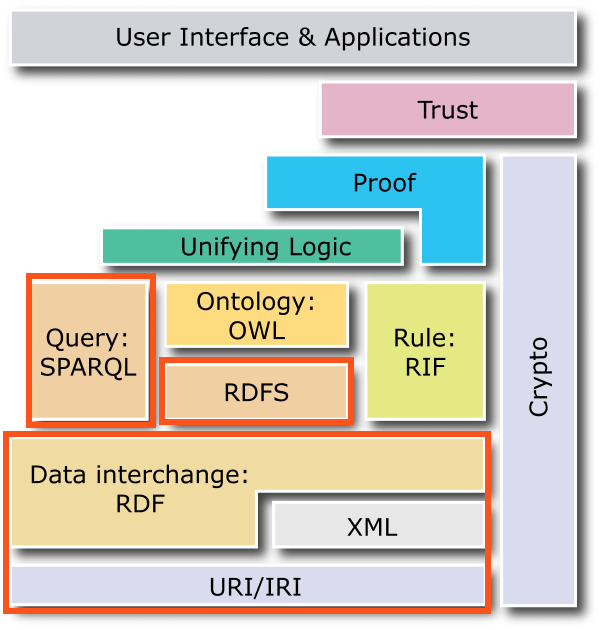
\includegraphics[width=160px]{Semantic_Web_Stack_rect.png} 
% \end{figure}
% \end{frame}

\begin{frame}
\frametitle{International Resource Identifier}

La specifica \emph{International Resource Identifier} (in breve \emph{IRI},
vedi RFC3987) estende quella per gli \emph{Uniform Resource Identifier} (in breve \emph{URI},
vedi RFC3986) con un pi\`u ampio repertorio di caratteri, aggiungendo
funzionalit\`a per l'internazionalizzazione.
\vspace{\baselineskip}

Nel seguito indicheremo con $\IRI$ l'insieme di tutti
i possibili IRI (i.e. l'insieme delle stringhe che rispettano la 
specifica IRI).
\end{frame}

\begin{frame}
\frametitle{IRI nel Web Semantico}
Nell'ambito del Web Semantico, tutti gli oggetti reali o concreti sono
identificati attraverso IRI. As esempio
\begin{center}
 \url{http://dbpedia.org/resource/Leonardo_da_Vinci}
\end{center}
\`e la IRI usata nell'ontologia \url{dbpedia.org} per indicare
Leonardo da Vinci, e ancora 
\begin{center}
  \begin{small}
    \url{http://data.europeana.eu/item/04802/243FA8618938F4117025F17A8B813C5F9AA4D619}
  \end{small}
\end{center}
indica la \emph{Mona Lisa} nell'ontologia del progetto \emph{Europeana}.
\end{frame}

\begin{frame}
\frametitle{IRI nel Web Semantico - \emph{Sinonimie}}
Si noti che una IRI \`e associata ad un unico oggetto, ma ad 
ogni oggetto possono essere associati diversi IRI.
\vspace{\baselineskip}

Ad esempio le seguenti IRI sono entrambe associate alla Monnalisa:
\vspace{\baselineskip}

\begin{small}
  \begin{tabular}{l}
      \url{http://data.europeana.eu/item/04802/243FA8618938F4117025F17A8B813C5F9AA4D619}\\
    \\
      \url{http://dbpedia.org/page/Mona_Lisa} .
  \end{tabular}
\end{small}
\end{frame}

\begin{frame}
\frametitle{Letterali}

I letterali vengono usati per rappresentare tipi di dato \emph{concreti},
come ad esempio stringhe di testo, numeri, date, \ldots
\vspace{\baselineskip}

Grazie ai letterali \`e possibile ad esempio esprimere affermazioni dei seguenti tipi:
\begin{itemize}
 \item Il cognome di Mario \`e \emph{Rossi};
 \item Cristiano \`e nato il giorno \emph{22 Marzo 1979};
 \item L'Empire State Building \`e alto \emph{380 metri}.
\end{itemize}
\end{frame}

\begin{frame}
\frametitle{Datatype}
Per introdurre i Letterali \`e necessario fornire prima la definizione di \emph{datatype}
(vedi \url{http://www.w3.org/TR/2014/REC-rdf11-concepts-20140225/\#section-Datatypes} e 
\url{http://www.w3.org/TR/xmlschema11-2/}).
\vspace{\baselineskip}

Un \emph{datatype} \`e caratterizzato da tre componenti:
\begin{itemize}
 \item un \emph{lexical space}, ossia un insieme di stringhe (finite) di caratteri nella codifica \emph{UNICODE};
 \item un \emph{value space}, che \`e un insieme non meglio specificato e numerabile di \emph{valori} (interi, date,
 Booleani, \ldots);
 \item un \emph{lexical-value mapping} che associa ad ogni stringa nel lexical space un elemento nel value space.
\end{itemize}
\vspace{\baselineskip}

I datatype vengono di solito indicati con delle IRI.
\end{frame}

\begin{frame}
\frametitle{Datatype - Esempio 1 : \url{xsd:integer}}
Il datatype \url{xsd:integer} (dove \url{xsd} \`e l'abbreviazione per il namespace \url{http://www.w3.org/2001/XMLSchema\#})
\`e definito come segue:

\begin{itemize}
 \item il \emph{lexical space} di \url{xsd:integer} \`e costituito da tutte le sequenze finite di cifre da 0 a 9, possibilmente
 precedute dal carattere ``-'' o ``+'';
 \item il \emph{value space} \`e l'insieme dei numeri interi;
 \item il valore di una stringa nel lexical space di \url{xsd:integer} si ottiene considerando le cifre 
 presenti nella stringa come cifre del corrispondente numero in base $10$, e moltiplicando il numero cos\`i ottenuto per
 $-1$ nel caso in cui la stringa inizi con il carattere ``-''.
\end{itemize}
\end{frame}

\begin{frame}
\frametitle{Datatype - Esempio 2 : \url{xsd:string}}
Il datatype \url{xsd:string} \`e definito come segue:

\begin{itemize}
 \item il \emph{lexical space} di \url{xsd:string} comprende 
 tutte le sequenze di caratteri (UNICODE) di zero o pi\`u caratteri;
 \item il \emph{value space} di \url{xsd:string} coincide col suo 
 lexical space;
 \item il \emph{lexical-value mapping} associa ogni stringa nel lexical space
 con se stessa (indetit\`a).
 \end{itemize}
\end{frame}

\begin{frame}
 \frametitle{Altri esempi di datatype}
Riportiamo alcuni datatype (mutuati da XML Schema) di uso comune.

\begin{small}
\begin{tabular}{|l|l|}
 \hline
\url{xsd:boolean} & true, false\\
\url{xsd:decimal} & Arbitrary-precision decimal numbers\\
\url{xsd:integer} & Arbitrary-size integer numbers\\
\url{xsd:double} & 64-bit floating point numbers incl. ±Inf, ±0, NaN\\
\url{xsd:float} & 32-bit floating point numbers incl. ±Inf, ±0, NaN\\
\url{xsd:date} & Dates (yyyy-mm-dd) with or without timezone\\
\url{xsd:time} & Times (hh:mm:ss.sss…) with or without timezone\\
\url{xsd:dateTime} & Date and time with or without timezone\\
\url{xsd:dateTimeStamp} & Date and time with required timezone\\
\url{xsd:duration} & Duration of time\\
\url{xsd:byte} & -128\ldots+127 (8 bit)\\
\url{xsd:short} & -32768\ldots+32767 (16 bit) \\
\url{xsd:int} & -2147483648\ldots+2147483647 (32 bit)\\
\url{xsd:long} & -9223372036854775808\ldots+9223372036854775807 (64 bit)\\
\url{xsd:unsignedByte} & 0\ldots255 (8 bit)\\
\url{xsd:unsignedShort} & 0\ldots65535 (16 bit)\\
\url{xsd:unsignedInt} & 0\ldots4294967295 (32 bit)\\
\url{xsd:unsignedLong} & 0\ldots18446744073709551615 (64 bit)\\
\url{xsd:positiveInteger} & Integer numbers $>0$\\
\url{xsd:nonNegativeInteger} & Integer numbers $\geq 0$\\
\url{xsd:negativeInteger} & Integer numbers $<0$\\
\url{xsd:nonPositiveInteger} & Integer numbers $\leq 0$\\
\url{xsd:hexBinary} & Hex-encoded binary data\\
\hline
\end{tabular}
\end{small}
\end{frame}

\begin{frame}
\frametitle{Letterali - Definizione}
Formalmente, i letterali sono definiti come segue (vedi 
\url{http://www.w3.org/TR/2014/REC-rdf11-concepts-20140225/\#section-Graph-Literal}).
\vspace{\baselineskip}

Un \emph{letterale} \`e costituito da un \emph{datatype} $t$ e da una 
stringa di caratteri nel lexical space di $t$ (la cosiddetta \emph{lexical form}
del letterale).
\vspace{\baselineskip}

Se un letterale \`e di tipo \url{xsd:string}, ad esso pu\`o essere associato un
\emph{language tag} ad indicarne la \emph{lingua}. Per i valori che questo attributo pu\`o
assumere fare riferimento allo \emph{IANA Language Subtag Registry}.
\end{frame}

\begin{frame}
\frametitle{Letterali - Esempi}
Seguono alcuni esempi di letterali:

\begin{center}
\begin{tabular}{|l|l|c|}
  \hline
  \textbf{lexical form} & \textbf{data type} & \textbf{language tag}\\
  \hline
  ``380'' & \url{xsd:integer} & - \\
  ``March-22-1979'' & \url{xsd:date} & - \\
  ``Rossi'' & \url{xsd:string} & - \\
  ``Parigi'' & \url{xsd:string} & it \\
  ``Paris'' & \url{xsd:string} & en\\
  \hline
\end{tabular}
\end{center}
\vspace{\baselineskip}

Nel caso in cui si ometta l'indicazione del tipo di dato, il letterale si assume essere
di tipo \url{xsd:string}.
\end{frame}


\begin{frame}
\frametitle{Letterali - Notazione (1/3)}
Per indicare i letterali spesso si usano le seguenti notazioni
\[
 \begin{array}{c}
   \literal{lexform}{type} \\
   \\
  < lexform, type >
 \end{array}
\]
ove $lexform$ e $type$ sono la lexical form e il data type del letterale, rispettivamente.
\vspace{\baselineskip}

Alcuni esempi:
\[
\begin{array}{ll}
 \literal{380}{xsd:integer} & <``380'', \mathtt{xsd:integer}>\\
 \literal{March-22-1979}{xsd:date} & <``March-22-1979'', \mathtt{xsd:date}>\\
 \literal{Rossi}{xsd:string} & <``Rossi'', \mathtt{xsd:string}>
\end{array}
\]
\end{frame}

\newcommand{\mathurl}[1]{\mbox{\url{#1}}}

\begin{frame}
\frametitle{Letterali - Notazione (3/3)}
Dato un letterale $l$, indicheremo con
\begin{itemize}
 \item $datatype(l)$ il tipo di dato di $l$, e con 
 \item $lexform(l)$ la lexical form di $l$.
\end{itemize}
\vspace{\baselineskip}

Seguono alcuni esempi:
\[
\begin{array}{l}
 datatype(\literal{380}{xsd:integer}) = \mathurl{xsd:integer}\\
 datatype(\literal{March-22-1979}{xsd:date}) = \mathurl{xsd:date}\\
 datatype(\literal{Rossi}{xsd:string}) = \mathurl{xsd:string}\\
 \\
 lexform(\literal{380}{xsd:integer}) = \stringLiteral{380}\\
 lexform(\literal{March-22-1979}{xsd:date}) = \stringLiteral{March-22-1979}\\
 lexform(\literal{Rossi}{xsd:string}) = \stringLiteral{Rossi} 
\end{array}
\]
\end{frame}


\begin{frame}
\frametitle{Confronto tra Letterali}
Due letterali sono uguali se e solo se sono uguali le loro lexical form,
se hanno lo stesso tipo e se sono uguali i loro language tag, ove presenti.
Di conseguenza due letterali possono essere diversi anche avendo lo stesso
\emph{valore}. Ad esempio i due seguenti letterali hanno entrambi 
come valore l'intero $1$ ma sono diversi:
\vspace{\baselineskip}

\[
 \begin{array}{l}
  \literal{1}{xsd:integer}\\
  \literal{01}{xsd:integer} .\\
 \end{array}
\]
\end{frame}

\begin{frame}
\frametitle{Property Assertions con Letterali}

I letterali possono essere usati per specificare \emph{propriet\`a} di un
individuo. In altre parole, essi possono comparire come \emph{oggetto}
di una property assertion. Alcuni esempi di role assertion che coinvolgono
letterali sono
\[
 \begin{array}{l}
  Mario \, surname \, \literal{Rossi}{xsd:string} \\
  Cristiano \, hasbirth \, \literal{March-22-1979}{xsd:date}\\
 \end{array}
\]
con $Mario, Cristiano \in \INames$, $surname, hasbirth \in \PNames$ e 
$\literal{Rossi}{xsd:string}$, $\literal{March-22-1979}{xsd:date}$ letterali.

\end{frame}

\begin{frame}
 \frametitle{Ontologie nel Web Semantico - Sintassi}

Siano $\CNames$, $\PNames$, $\INames$, $\DNames$, $\literals$ insiemi
infiniti, numerabili e a due a due disgiunti di nomi di \emph{classe}, \emph{propriet\`a},
\emph{individuo} e di  \emph{datatype} e di \emph{letterali}, rispettivamente,
tali che
\[
	\CNames \cup \PNames \cup \INames \cup \DNames \subseteq \IRI , 
\]
e $\literals$ siano i letterali (nel senso visto prima) i cui datatype
sono in $\DNames$.

Una \emph{ontologia} \`e un insieme finito di asserzioni dei seguenti tipi:
\[
 \begin{array}{ll}
  \mbox{(Constraints)} & C \Issub D\\
  & P \Issub Q \\
  & \dom(P) \Issub C \\
  & \range(P) \Issub C \\
  &\\
  \mbox{(Class Assertions)} & C(a)\\
  &\\
  \mbox{Property Assertions} & a\,P\,b\\
  & \mathbf{a\,P\,l}\\
 \end{array}
\]
dove $C, D \in \CNames$, $P, Q \in \PNames$, $a, b \in \INames$,
e $l \in \LNames$.
\end{frame}

\begin{frame}
 \frametitle{Ontologie - Semantica}
Una \emph{interpretazione} \`e una
tripla $\I=(\Delta^{\I}$, $\Delta_{D}^{\I}$, $\cdot^{\I})$ dove:
\begin{itemize}
 \item $\Delta^{\I}, \Delta_{D}^{\I}$ sono due insiemi disgiunti e non vuoti;
 \item $\cdot^{\I}$ \`e una funzione (polimorfa) che associa
 \begin{itemize}
  \item ad ogni nome di concetto $C$ in $\CNames$ un sottoinsieme $C^{\I}$ di
  $\Delta^{\I}$,
  \item ad ogni datatype $t$ un sottoinsieme di $t^{\I}$ di $\Delta_{D}$, 
  \item ad ogni nome di propriet\`a in $P$ in $\PNames$ una relazione 
  $P^{\I} \subseteq \Delta^{\I} \times (\Delta^{\I} \cup \Delta_D^{\I})$,
  \item ad ogni nome di individuo $a$ in $\INames$ un elemento $a^{\I}$ di
  $\Delta^{\I}$,
  \item ad ogni letterale $l$ in $\literals$ un elemento in $t^{\I}$, ove
  $t=datatype(l)$.
 \end{itemize}
\end{itemize}

Le nozione di soddisfacibilit\`a di una ontologia e di implicazione di 
ontologie seguono da questa nuova definizione.
\end{frame}


\begin{frame}
\frametitle{Ontologie con Letterali - Esempio}
Consideriamo come esempio il vocabolario $\Vocab$ definito come segue:
\[
 \begin{array}{rcl}
  \Vocab & \defAs & (C, P, \Omega) \\
  C & \defAs & \{Person\}\\
  P & \defAs & \{childOf, fullName, age\}\\
  \Omega & \defAs & \{\dom(childOf) \Issub Person, \range(childOf) \Issub Person, \\
  &&\phantom{\{} \dom(fullName) \Issub Person, \range(fullName) \Issub xsd:string \\
  &&\phantom{\{} \dom(age) \Issub Person, \range(age) \Issub xsd:nonNegativeInteger \} ,
 \end{array}
\]
e l'ontologia con letterali $\Ont$ costruita a partire da $\Vocab$
\[
 \begin{array}{rcl}
  \Ont & \defAs & \Omega \cup \{ Person(Eliza), Person(Alice), Person(Bob),\\
  &&\phantom{\Omega \cup \{}Alice\,childOf\,Eliza, Bob\,childOf\,Eliza\\
  &&\phantom{\Omega \cup \{}Eliza\,fullName\, \stringLiteral{Eliza Smith}, Eliza\,age\,\literal{63}{xsd:nonNegativeInteger} \}\\
 \end{array}
\]

\end{frame}

\begin{frame}
\frametitle{Ontologie con Letterali - Alcune notazioni}
Data una qualsiasi ontologia (con letterali) $\Ont$, indicheremo con:
\begin{itemize}
 \item $\CNames(\Ont)$ l'insieme dei nomi di concetto che compaiono in $\Ont$;
 \item $\PNames(\Ont)$ l'insieme dei nomi di propriet\`a che compaiono in $\Ont$;
 \item $\INames(\Ont)$ l'insieme dei nomi di individuo che compaiono in $\Ont$;
 \item $\literals(\Ont)$ l'insieme dei letterali che compaiono in $\Ont$.
\end{itemize}
\vspace{\baselineskip}

Definizioni analoghe si applicano ai vocabolari.
\vspace{\baselineskip}

Inoltre, indichiamo con $\IRI$ l'insieme di tutti i possibili IRI.
\end{frame}

\section{RDF}

\begin{frame}
 \frametitle{Resource Description Framework (RDF)}
 Il \emph{linguaggio di rappresentazione} pi\`u basilare nella pila
 delle tecnologie del Web Semantico \`e il cosiddetto 
 \emph{Resource Description Framework} (nel seguito \emph{RDF}).
 
%  \begin{figure}
%  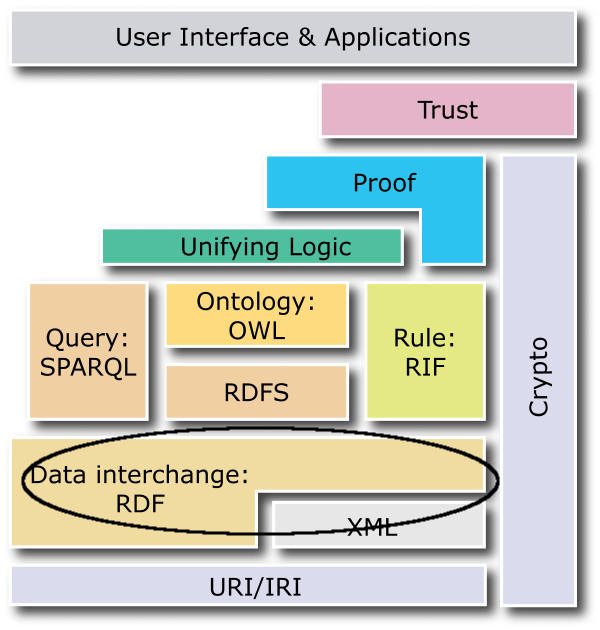
\includegraphics[width=160px]{Semantic_Web_Stack_RDF.png} 
%  \end{figure}
\end{frame}

\newcommand{\RDFv}{\mathtt{RDF}}

\begin{frame}
 \frametitle{Vocabolario RDF}
 Il \emph{vocabolario $\RDFv$} pu\`o essere definito come segue:
 
\[
 \begin{array}{cclc}
 \RDFv & \defAs & (C_{RDF}, P_{RDF}, \Omega_{RDF}) \\
 &&\\
 C_{RDF} & \defAs & \{\mathurl{rdf:Property}, \mathurl{rdf:List}\}\\
 &&\\
 P_{RDF} & \defAs & \{\mathurl{rdf:type}, \mathurl{rdf:subject}, \mathurl{rdf:predicate}, \mathurl{rdf:object},\\
 && \phantom{\{} \mathurl{rdf:first}, \mathurl{rdf:rest}, \mathurl{rdf:value}, \mathurl{rdf:_1}, \mathurl{rdf:_2}, \ldots \}\\ 
 \\
 \Omega_{RDF} & \defAs & \{ (\forall a, C)(a\,\mathurl{rdf:type}\,C \leftrightarrow C(a)), & (*)\\ 
 &&\phantom{\{}(\forall a,P,b)(a\,P\,b \rightarrow \mathurl{rdf:Property}(P)), & (**) \\
 &&\phantom{\{}\range(\mathurl{rdf:first}) \Issub \mathurl{rdf:List},\\
 &&\phantom{\{}\range(\mathurl{rdf:rest}) \Issub \mathurl{rdf:List} \, \}\\
 \end{array}
\]
dove il prefisso \url{rdf:} \`e una abbreviazione per il namespace
\begin{center}
 \url{http://www.w3.org/1999/02/22-rdf-syntax-ns\#}
\end{center}
\vspace{\baselineskip}

Il vocabolario $\RDFv$ definisce inoltre un nome di individuo \url{rdf:nil}, 
appartenente alla class \url{rdf:List}, ed il datatype \url{rdf:XMLLiteral},
che indica un frammento XML.
\vspace{\baselineskip}

\uncover<2>{
Peculiarit\`a di $\RDFv$ :
\begin{itemize}
 \item L'insieme $P_{RDF}$ \`e infinito.
 \item I vincoli $(*)$ e $(**)$ non sono esprimibili nelle ontologie, servono a definire
 la \emph{semantica} del linguaggio RDF.
\end{itemize}
}
\end{frame}

\begin{frame}
 \frametitle{Grafi RDF}
 Un \emph{grafo RDF} \`e un insieme finito di property assertions dei seguenti tipi:
\[
 \begin{array}{rcl}
  a & P & b \\
  a & P & l
 \end{array}
\]
con 
\[
 \begin{array}{l}
 P \in \IRI\\
 a, b \in \IRI \cup \BlankNodes\\
 l \in \literals
 \end{array}
\]
per qualche insieme $\BlankNodes$ disgiunto da $\IRI$.
\vspace{\baselineskip}

\uncover<2>{
Dato un grafo RDf $G$, gli elementi di $\BlankNodes$ che compaiono in $G$ sono
definiti \emph{blank node} di $G$. Indicheremo con
$\BlankNodes(G)$ l'insieme dei blank node del grafo $G$.
}
\end{frame}

\newcommand{\triple}[3]{\mathurl{#1}\;\mathurl{#2}\;#3}
\newcommand{\tripleO}[3]{\mathurl{#1}\;\mathurl{#2}\;\mathurl{#3}}

\begin{frame}
 \frametitle{Grafi RDF - Esempio}
 Un esempio di grafo RDF \`e il seguente:
 \[
 \begin{array}{rcl}
  G & \defAs & \{ \tripleO{ex:Eliza}{rdf:type}{ex:Person},\\
  &&\phantom{\{} \tripleO{ex:Alice}{rdf:type}{ex:Person},\\
  &&\phantom{\{} \tripleO{ex:Bob}{rdf:type}{ex:Person},\\
  \\
  &&\phantom{\{} \tripleO{ex:childOf}{rdf:type}{rdf:Property},\\
  &&\phantom{\{} \tripleO{ex:fullName}{rdf:type}{rdf:Property},\\
  &&\phantom{\{} \tripleO{ex:age}{rdf:type}{rdf:Property},\\
  \\
  &&\phantom{\{} \tripleO{ex:Alice}{ex:childOf}{ex:Eliza},\\
  &&\phantom{\{} \tripleO{ex:Bob}{ex:childOf}{ex:Eliza},\\
  &&\phantom{\{} \triple{ex:Eliza}{ex:fullName}{\stringLiteral{Eliza Smith}},\\
  &&\phantom{\{} \triple{ex:Eliza}{ex:age}{\literal{63}{xsd:nonNegativeInteger}} \,\},\\
 \end{array}
\]
\end{frame}

\begin{frame}
 \frametitle{Ontologie RDF}
 Dato un grafo RDF $G$, la corrispondente ontologia RDF $\Ont_G$ \`e ottenuta come segue:
 \[
  \Ont_G \defAs \Omega_{RDF} \cup G .
 \]
 
\uncover<2>{
 Da questa definizione e dal fatto che un grafo RDF 
 \`e un insieme finito di property assertions dei seguenti tipi:
\[
 \begin{array}{rcl}
  a & P & b \\
  a & P & l
 \end{array}
\]
con $P \in \IRI$, $a, b \in \IRI \cup \BlankNodes$ e $l \in \literals$, 
per qualche insieme $\BlankNodes$ disgiunto da $\IRI$,
segue che
\[
 \begin{array}{rcl}
  \CNames(\Ont_G) & \subseteq & \IRI\\
  \PNames(\Ont_G) & \subseteq & \IRI\\  
  \INames(\Ont_G) & \subseteq & \IRI \cup \BlankNodes
 \end{array}
\]
per ogni grafo RDF $G$ e per la corrispondente ontologia RDF $\Ont_G$.
}
\end{frame}

\begin{frame}
 \frametitle{Class assertions in RDF}
 Asserzioni del tipo $a\, \mathurl{rdf:type}\,C$ vengono usate in RDF 
 per affermare class assertions $C(a)$.
 \vspace{\baselineskip}
 
 Infatti, grazie al vincolo presente in $\Omega_{RDF}$
 \[
  (\forall a, C)(a\,\mathurl{rdf:type}\,C \leftrightarrow C(a)) \quad(*).
 \]
 da ogni asserzione del tipo $a\, \mathurl{rdf:type}\,C$ tramite reasoning
 viene inferita una asserzione $C(a)$.
 \vspace{\baselineskip}
 
 Consideriamo ad esempio il grafo RDF $G$ visto prima e la corrispondente 
 ontologia RDF:
 \[
 \begin{small}
 \begin{array}{lcl}
  \Omega_{RDF} \cup \{ \tripleO{ex:Eliza}{rdf:type}{ex:Person},&&\{ \mathurl{ex:Person}(\mathurl{ex:Eliza}),\\
  \phantom{\{} \tripleO{ex:Alice}{rdf:type}{ex:Person},&&\phantom{\{}\mathurl{ex:Person}(\mathurl{ex:Alice}),\\
  \phantom{\{} \tripleO{ex:Bob}{rdf:type}{ex:Person},&&\phantom{\{}\mathurl{ex:Person}(\mathurl{ex:Bob}),\\
  \phantom{\{} \tripleO{ex:childOf}{rdf:type}{rdf:Property},& \Longrightarrow & \phantom{\{}\mathurl{ex:Property}(\mathurl{ex:childOf}),\\
  \phantom{\{} \tripleO{ex:fullName}{rdf:type}{rdf:Property},&&\phantom{\{}\mathurl{ex:Property}(\mathurl{ex:fullName}),\\
  \phantom{\{} \tripleO{ex:age}{rdf:type}{rdf:Property},&&\phantom{\{}\mathurl{ex:Property}(\mathurl{ex:age}),\}\\
  \phantom{\{} \tripleO{ex:Alice}{ex:childOf}{ex:Eliza},&&\phantom{\{}\ldots \, \}\\
  \phantom{\{} \tripleO{ex:Bob}{ex:childOf}{ex:Eliza},\\
  \phantom{\{} \triple{ex:Eliza}{ex:fullName}{\stringLiteral{Eliza Smith}},\\
  \phantom{\{} \triple{ex:Eliza}{ex:age}{\literal{63}{xsd:nonNegativeInteger}} \,\},\\
\end{array}
\end{small}
\]
\end{frame}

\begin{frame}
 \frametitle{La classe \url{rdf:Property}}
Il seguente vincolo, presente in $\Omega_{RDF}$, garantisce che ogni 
propriet\`a $P$ presente in un grafo RDF sia riconosciuta come
istanza della classe \url{rdf:Property} 
\[
  (\forall a,P,b)(a\,P\,b \rightarrow \mathurl{rdf:Property}(P)) \quad (**)
\]

\uncover<2>{
Consideriamo ad esempio un grafo RDF $G$ e la corripondente ontologia $\Ont_G = \Omega_{RDF} \cup G$,
e sia $\Ont_G^{'}$ l'ontologia ottenuta estendendo $\Ont_G$ con le asserzioni
che si possono inferire da $\Ont_G$ tramite reasoning.

Supponiamo che la seguente asserzione sia in $G$. 
\[
 \tripleO{ex:Bob}{ex:childOf}{ex:Eliza} .
\]
Allora
\[
 \begin{array}{ll}
 \tripleO{ex:Bob}{ex:childOf}{ex:Eliza} \in G & \Longrightarrow \\
 \tripleO{ex:Bob}{ex:childOf}{ex:Eliza} \in \Ont_G & \Longrightarrow \\
 \tripleO{ex:Bob}{ex:childOf}{ex:Eliza} \in \Ont_G^{'} & \Longrightarrow (**)\\ %TODO overset
 \mathurl{rdf:Property}(\mathurl{ex:childOf}) \in \Ont_G^{'} & \Longrightarrow (*) \\ %TODO overset
 \tripleO{ex:childOf}{rdf:type}{rdf:Property} \in \Ont_G^{'}\\
 \end{array}
\]
}
\end{frame} 

\begin{frame}
 \frametitle{Vocabolari basati su RDF}
 Si noti che le propriet\`a in RDF sono trattate sia come propriet\`a che
 come \emph{individui}, inquanto istanze della classe \url{rdf:Property}.
 In altre parole, nel contesto RDF
 \[
  \PNames \subseteq \CNames .
 \]
 \vspace{\baselineskip}
 
 Operazioni di questo tipo sono in genere \emph{rischiose} in termini 
 di indecidibilit\`a (vedi OWL Full).   
 \vspace{\baselineskip}

 In genere, la natura di individuo di una propriet\`a viene utilizzata
 solo nella realizzazione di vocabolari, per \emph{annotare} le propriet\`a
 con commenti ed etichette esplicative oppure per descrivere i vincoli,
 come vedremo più avanti.
\end{frame} 

% \section{Serializzazioni}
% 
\begin{frame}
 \frametitle{Serializzazione di grafi RDF}
 
 Il processo di serializzazione di un grafo RDF permette
 di scrivere un grafo su un file o di inviarlo in rete.
 \vspace{\baselineskip}
 
 La serializzazione di un grafo RDF genera una stringa di testo
 in una delle seguenti \emph{sintassi concrete}:
 \begin{itemize}
  \item NTriples
  \item Turle
  \item RDF XML
  \item RDFa
  \item ...
 \end{itemize}
\end{frame} 

\begin{frame}[fragile]
 \frametitle{La Sintassi RDF N-Triples}
 
 Un grafo RDF serializzato secondo la sintassi N-Triples \`e
 una sequenza di righe con la seguente sintassi
\[
\begin{array}{rcl}
 r & := & <IRI> \quad <IRI> \quad o . \\
 o & := & <IRI> | \stringLiteral{STRING} | \literal{STRING}{<IRI>}
\end{array} 
\]
dove $IRI$ sono delle IRI e $STRING$ stringhe UNICODE.
\vspace{\baselineskip}

Intuitivamente, ogni riga di un file N-Triples rappresenta 
una property assertion RDF. Nel seguito un esempio di grafo
RDF espresso in N-Triples.
\vspace{\baselineskip}


\begin{Verbatim}[fontsize=\small]
<http://ex.org/Alice> <http://ex.org/childOf> <http://ex.org/Eliza> .
<http://ex.org/Bob> <http://ex.org/childOf> <http://ex.org/Eliza> .
<http://ex.org/Bob> <http://ex.org/childOf> <http://ex.org/Eliza> .
<http://ex.org/Eliza> <http://ex.org/fullName> "Eliza Smith" .
<http://ex.org/Eliza> <http://ex.org/age> 
                        "63"^^<http://www.w3.org/2001/XMLSchema#nonNegativeInteger> .
\end{Verbatim}
\end{frame}

\begin{frame}[fragile]
 \frametitle{La Sintassi RDF Turle - Predicate List}
 
\emph{Turtle} estende N-Triples con alcune funzionalit\`a.
\vspace{\baselineskip}

\emph{Predicate List} - Usando il simbolo ``;'' al posto di ``.'' al termine di alcune righe \`e possibile
specificare coppie [predicato, oggetto] che si riferiscono allo stesso soggetto. Ad esempio, le seguenti
righe (N-Triples)

\begin{Verbatim}[fontsize=\small]
<http://ex.org/Eliza> <http://ex.org/childOf> <http://ex.org/Giorgia> .
<http://ex.org/Eliza> <http://ex.org/childOf> <http://ex.org/Francis> .
<http://ex.org/Eliza> <http://ex.org/fullName> "Eliza Smith" .
<http://ex.org/Eliza> <http://ex.org/age> 
                        "63"^^<http://www.w3.org/2001/XMLSchema#nonNegativeInteger> .
\end{Verbatim}

possono essere espresse in Turtle come segue:
\begin{Verbatim}[fontsize=\small]
<http://ex.org/Eliza> <http://ex.org/childOf> <http://ex.org/Giorgia> ;
                      <http://ex.org/childOf> <http://ex.org/Francis> ;
                      <http://ex.org/fullName> "Eliza Smith" ;
                      <http://ex.org/age> 
                         "63"^^<http://www.w3.org/2001/XMLSchema#nonNegativeInteger> .
\end{Verbatim}
\end{frame}

\begin{frame}[fragile]
 \frametitle{La Sintassi RDF Turle - Object List}
Analogamente, usando simbolo ``,'' al posto di ``.'' al termine di alcune righe \`e possibile
specificare molteplici \emph{oggetti} che si riferiscono alla stessa coppia [soggetto, predicato]
Ad esempio

\begin{Verbatim}[fontsize=\small]
<http://ex.org/Eliza> <http://ex.org/childOf> <http://ex.org/Giorgia> .
<http://ex.org/Eliza> <http://ex.org/childOf> <http://ex.org/Francis> .
\end{Verbatim}

possono essere abbreviate con
\begin{Verbatim}[fontsize=\small]
<http://ex.org/Eliza> <http://ex.org/childOf> <http://ex.org/Giorgia> ,
                                              <http://ex.org/Francis> .
\end{Verbatim}
\end{frame}
 
% \begin{frame}[fragile]
%  \frametitle{La Sintassi RDF Turle - Prefisso base}
% 
% Con la parola chiave base \`e possibile specificare un \emph{prefisso base}
% che verr\`a utilizzato per risolvere le IRI incomplete presenti nel grafo RDF.
% 
% \begin{Verbatim}[fontsize=\small]
% @base <http://ex.org/>
% 
% <Eliza> <childOf> <Giorgia> ;
%         <childOf> <Francis> ;
%          <fullName> "Eliza Smith" ;
%          <age> "63"^^<http://www.w3.org/2001/XMLSchema#nonNegativeInteger> .
% \end{Verbatim}
% \end{frame}

\begin{frame}[fragile]
 \frametitle{La Sintassi RDF Turle - Prefisso base}

Con la parola chiave base \`e possibile specificare un \emph{prefisso base}
che verr\`a utilizzato per risolvere le IRI incomplete presenti nel grafo RDF.

\begin{Verbatim}[fontsize=\small]
BASE <http://ex.org/> .

<Eliza> <childOf>  <Giorgia> ,
                   <Francis> .
<Eliza> <fullName> "Eliza Smith" ;
        <age> "63"^^<http://www.w3.org/2001/XMLSchema#nonNegativeInteger> .
\end{Verbatim}
\end{frame}

\begin{frame}[fragile]
 \frametitle{La Sintassi RDF Turle - Prefissi}

\`E possibile inoltre dichiarare anche altri \emph{prefissi} da utilizzare
per abbreviare le IRI.

\begin{Verbatim}[fontsize=\small]
BASE <http://ex.org/>
PREFIX rdf: <http://www.w3.org/1999/02/22-rdf-syntax-ns#>
PREFIX xsd: <http://www.w3.org/2001/XMLSchema#> .

<Eliza>   <rdf:type> <Person> .
<Giorgia> <rdf:type> <Person> .
<Francis> <rdf:type> <Person> .
<Eliza>   <childOf>  <Giorgia> ,
                     <Francis> . 
<Eliza>   <fullName> "Eliza Smith" ;
          <age>      "63"^^<xsd:nonNegativeInteger> .
\end{Verbatim}
\end{frame}

\begin{frame}[fragile]
 \frametitle{La Sintassi RDF Turle - \url{rdf:type}}

Il simbolo 'a' pu\`o essere usato al posto del predicato \url{rdf:type}.

\begin{Verbatim}[fontsize=\small]
BASE <http://ex.org/> .
PREFIX rdf: <http://www.w3.org/1999/02/22-rdf-syntax-ns#> .
PREFIX xsd: <http://www.w3.org/2001/XMLSchema#> .

<Eliza> a <Person> .
<Giorgia> a <Person> .
<Francis> a <Person> .
<Eliza> <childOf> <Giorgia> ,
                  <Francis> .
<Eliza>  <fullName> "Eliza Smith" ;
         <age> "63"^^<xsd:nonNegativeInteger> .
\end{Verbatim}
\end{frame}

\begin{frame}[fragile]
 \frametitle{La Sintassi RDF Turle - Letterali}

Turtle definisce alcune abbreviazioni anche per i letterali,
che permettono di non indicare esplicitamente il data type.
Ad esempio:

\begin{Verbatim}[fontsize=\small]
BASE <http://ex.org/>

<http://en.wikipedia.org/wiki/Helium>                                                                                  
    :atomicNumber 2 ;               # xsd:integer                                                                      
    :atomicMass 4.002602 ;          # xsd:decimal                                                                      
    :specificGravity 1.663E-4 .     # xsd:double   
\end{Verbatim}
\vspace{\baselineskip}

Per un elenco completo delle abbreviazioni disponibili in Turtle per i
letterali fare riferimento a \url{http://www.w3.org/TR/2014/REC-turtle-20140225/\#literals} .
\end{frame}

\begin{frame}
 \frametitle{La Sintassi RDF XML}
 La sintassi \emph{RDF XML} permette di serializzare un grafo RDF 
 in un documento XML. L'elemento radice di questo documento \`e di
 tipo \url{rdf:RDF}.
 \vspace{\baselineskip}
 
 Gli elementi figli della radice sono di tipo \url{rdf:Description}
 e rappresentano \emph{nodi} del grafo RDF (individui). La IRI associata 
 al nodo viene specificata con l'attributo \url{rdf:about}. Nel caso in
 cui non sia presente l'attributo \url{rdf:about} siamo in presenza
 di un blank node.
 \vspace{\baselineskip}

 I figli di ogni elemento di tipo \url{rdf:Description} sono le
 propriet\`a con le quali sono etichettati gli archi uscenti dal 
 nodo che stiamo rappresentando.
 \vspace{\baselineskip}

 A loro volta, tali elementi rappresentanti gli archi uscenti da
 un nodo possono avere come figli 
 \begin{itemize}
  \item altri elementi di tipo \url{rdf:Description}, nel caso in cui
  l'oggetto della asserzione sia un individuo,
  \item degli elementi con un datatype come tipo, nel caso in cui 
  l'oggetto della asserzione sia un letterale,
  \item oppure possono avere un attributo \url{rdf:resource} che ha
  come valore la IRI associata all'individuo oggetto dell'asserzione.
 \end{itemize}
\end{frame}

\begin{frame}[fragile]
 \frametitle{La Sintassi RDF XML - Property assertions}
 In altre parole, una property assertion del tipo $\tripleO{iriSubj}{iriProp}{iriObj}$,
 con $iriSubj, iriProp, iriObj$ pu\`o essere serializzata in RDF XML 
 con il seguente elemento 

 \begin{Verbatim}[fontsize=\small]
   <rdf:Description rdf:about="iriSubj">
     <iriProp>
       <rdf:Description rdf:about="iriObj" />
     <iriProp>      
   </rdf:Description>
\end{Verbatim}

oppure, utilizzando \url{rdf:resource}, con

\begin{Verbatim}[fontsize=\small]
   <rdf:Description rdf:about="iriSubj">
     <iriProp rdf:resource="iriObj" />
   </rdf:Description>
\end{Verbatim}
\end{frame}

\begin{frame}[fragile]
 \frametitle{La Sintassi RDF XML - Multiple Property assertions}
 
 
 Inoltre, property assertions con lo stesso oggetto possono essere 
 raggruppate all'interno di un unico elemento di tipo \url{rdf:Description}.
 Vediamo ad esempio una possibile serializzazione in RDF XML di due asserzioni 
 con lo stesso soggetto.
\[
\begin{array}{l}
 iriSubj\,iriProp1\,iriObj1 \,, \\
 iriSubj\,iriProp2\,iriObj2
\end{array}
\]

\begin{Verbatim}[fontsize=\small]
   <rdf:Description rdf:about="iriSubj">
     <iriProp1 rdf:resource="iriObj1" />
     <iriProp2 rdf:resource="iriObj1" />
   </rdf:Description>
\end{Verbatim}
\end{frame}

% \begin{frame}[fragile]
%  \frametitle{La Sintassi RDF XML - Multiple Property assertions (2/)}
% Property assertions con lo stesso soggetto e predicato possono essere 
% raggruppate in maniera analoga.
% 
% \[
% \begin{array}{l}
%  iriSubj\,iriProp\,iriObj1 \,, \\
%  iriSubj\,iriProp\,iriObj2
% \end{array}
% \]
% 
% \vspace{\baselineskip}
% 
% \begin{Verbatim}[fontsize=\small]
%    <rdf:Description rdf:about="iriSubj">
%      <iriProp>
%        <rdf:Description rdf:about="iriSubj1" />
%        <rdf:Description rdf:about="iriSubj2" />
%      </iriProp>
%    </rdf:Description>
% \end{Verbatim}
% \end{frame}

\begin{frame}[fragile]
 \frametitle{La Sintassi RDF XML - String literals}
I letterali di tipo stringa specificati come oggetto di una 
properti assertions vanno inseriti come contenuto (CDATA) dell'elemento
che identifica la propriet\`a all'interno degli elementi \url{rdf:Description}.

Ad esempio una asserzione del tipo seguente
\[
 \triple{iriSubj}{iriProp}{\stringLiteral{string}}
\]
pu\`o essere serializzata come segue:
\vspace{\baselineskip}

\begin{Verbatim}[fontsize=\small]
   <rdf:Description rdf:about="iriSubj">
     <iriProp>string</iriProp>
   </rdf:Description>
\end{Verbatim}
\end{frame}

\begin{frame}[fragile]
 \frametitle{La Sintassi RDF XML - Datatype property}
\`E possibile inoltre specificare esplicitamente il datatype di un
letterale oggetto di una property assertion mediante l'attributo \url{rdf:datatype}.

\[
 \triple{iriSubj}{iriProp}{\literal{lexForm}{iriType}}
\]
\vspace{\baselineskip}

\begin{Verbatim}[fontsize=\small]
   <rdf:Description rdf:about="iriSubj">
     <iriProp rdf:datatype="iriType">lexForm</iriProp>
   </rdf:Description>
\end{Verbatim}
\end{frame}

\begin{frame}[fragile]
 \frametitle{La Sintassi RDF XML - Namespace}
Le abbreviazioni per i prefissi possono essere implementate attraverso
i meccanismi forniti dalla specifica XML. Segue un esempio completo
di grafo RDF serializzato in RDF/XML.
\vspace{\baselineskip}

\begin{Verbatim}[fontsize=\small]
<?xml version="1.0"?>
<rdf:RDF xmlns="http://ex.org/"
  xmlns:rdf="http://www.w3.org/1999/02/22-rdf-syntax-ns#"
  xmlns:xsd="http://www.w3.org/2001/XMLSchema#">

  <rdf:Description rdf:about="Giorgia">
    <rdf:type rdf:resource="http://ex.org/Person" />
  </rdf:Description>

  <rdf:Description rdf:about="Francis">
    <rdf:type rdf:resource="http://ex.org/Person" />
  </rdf:Description>
  
  <rdf:Description rdf:about="Eliza">
    <rdf:type rdf:resource="http://ex.org/Person" />
    <childOf>
      <rdf:Description rdf:about="Giorgia" />
      <rdf:Description rdf:about="Francis" />
    </childOf>    
    <fullName>Eliza Smith</fullName>
    <age rdf:datatype="http://www.w3.org/2001/XMLSchema#nonNegativeInteger">63</age>
  </rdf:Description>
</rdf:RDF>
\end{Verbatim}
\end{frame}

\begin{frame}[fragile]
 \frametitle{La Sintassi RDF XML - Typed Node Elements}
 
Se un individuo appartiene ad una classe con  
una qualche IRI $uriClass$, ossia se una una tripla del 
tipo
\[
 uriInd\,\mathurl{rdf:type}\,uriClass
\]
compare nel grafo RDF, \`e possibile non usare \url{rdf:Description}
per indicare l'individuo $uriInd$, ma al suo posto dichiarare
nel documento XML un elemento di tipo $uriClass$.
\vspace{\baselineskip}

Ad esempio, e seguenti due serializzazioni sono equivalenti.

\begin{Verbatim}[fontsize=\small]
  <rdf:Description rdf:about="Eliza">
    <rdf:type rdf:resource="http://ex.org/Person" />
    <childOf rdf:resource="http://ex.org/Giorgia" />
    <childOf rdf:resource="http://ex.org/Francis" />
    <fullName>Eliza Smith</fullName>
    <age rdf:datatype="http://www.w3.org/2001/XMLSchema#nonNegativeInteger">63</age>
  </rdf:Description>
\end{Verbatim}

\begin{Verbatim}[fontsize=\small]
  <Person rdf:about="Eliza">
    <childOf rdf:resource="http://ex.org/Giorgia" />
    <childOf rdf:resource="http://ex.org/Francis" />
    <fullName>Eliza Smith</fullName>
    <age rdf:datatype="http://www.w3.org/2001/XMLSchema#nonNegativeInteger">63</age>
  </Person>
\end{Verbatim}
\end{frame}

\section{RDFS}

\newcommand{\RDFSv}{\mathtt{RDFS}}

\begin{frame}
 \frametitle{RDF Schema}
 \emph{RDF Schema} (in breve \emph{RDFS}) estende RDF con 
 delle funzionalit\`a utili a definire nuovi vocabolari.
  \vspace{\baselineskip}

Il \emph{vocabolario $\RDFSv$} pu\`o essere definito come segue:
 
\[
 \begin{small}
 \begin{array}{cclc}
 \RDFSv & \defAs & (C_{RDFS}, P_{RDFS}, \Omega_{RDFS}) \\
 &&\\
 C_{RDFS} & \defAs & C_{RDF} \cup \{ \mathurl{rdfs:Resource}, \mathurl{rdfs:Literal}, \mathurl{rdfs:Datatype}, \\
 &&\phantom{C_{RDF} \cup \{}\mathurl{rdfs:Class}, \mathurl{rdfs:Container}, \mathurl{rdfs:ContainerMembershipProperty} \}\\
 &&\\
 P_{RDFS} & \defAs & P_{RDF} \cup \{\mathurl{rdfs:domain}, \mathurl{rdfs:range}, \mathurl{rdfs:subClassOf}, \mathurl{rdfs:subPropertyOf},\\
 &&\phantom{P_{RDF} \cup \{} \mathurl{rdfs:comment}, \mathurl{rdfs:seeAlso}, \mathurl{rdfs:isDefinedBy}, \mathurl{rdfs:label} \}\\
 \\
 \Omega_{RDFS} & \defAs & \Omega_{RDF} \cup \{ (\forall a, C)(C(a) \rightarrow a\,\mathurl{rdf:type}\,\mathurl{rdfs:Class}), & \\ 
 &&\phantom{\Omega_{RDFS} \cup \{}(\forall a,P,s,t)(a\,P\,\literal{s}{t} \rightarrow \literal{s}{t}\,\mathurl{rdf:type}\,\mathurl{rdfs:Literal}), & \\
 &&\phantom{\Omega_{RDFS} \cup \{}(\forall a,P,s,t)(a\,P\,\literal{s}{t} \rightarrow t\,\mathurl{rdf:type}\,\mathurl{rdfs:Datatype}), & \\
 &&\phantom{\Omega_{RDFS} \cup \{}(\forall C,D)(C\,\mathurl{rdfs:subClassOf}\,D  \leftrightarrow C \Issub D), & \\
 &&\phantom{\Omega_{RDFS} \cup \{}(\forall R,S)(R\,\mathurl{rdfs:subPropertyOf}\,S  \leftrightarrow R \Issub S), & \\
 &&\phantom{\Omega_{RDFS} \cup \{}(\forall R,C)(R\,\mathurl{rdfs:domain}\,C  \leftrightarrow \dom(R) \Issub C), & \\
 &&\phantom{\Omega_{RDFS} \cup \{}(\forall R,C)(R\,\mathurl{rdfs:range}\,C  \leftrightarrow \range(R) \Issub C)\,\} \\
 \end{array}
 \end{small}
\]
dove il prefisso \url{rdfs} \`e una abbreviazione per il namespace
\begin{center}
 \url{http://www.w3.org/2000/01/rdf-schema\#}
\end{center}
\end{frame}

\begin{frame}[fragile]
 \frametitle{Gerarchie di Classi e Propriet\`a}
 In RDFS \`e possibile definire gerarchie di classi. Nel seguito mostriamo alcuni esempi
 con la sintassi RDF XML.

\begin{Verbatim}[fontsize=\small]
<rdfs:Class rdf:about="http://ex.org/Man">
  <rdfs:subClassOf rdf:resource="http://ex.org/Person" />
</rdf:Class>

<rdfs:Class rdf:about="http://ex.org/Woman">
  <rdfs:subClassOf rdf:resource="http://ex.org/Person" />
</rdf:Class>

<rdf:Property rdf:about="http://ex.org/son">
  <rdfs:subPropertyOf rdf:resource="http://ex.org/childOf" />
</rdf:Property>
\end{Verbatim} 
\end{frame}

\begin{frame}[fragile]
 \frametitle{Annotazioni}
 \`E inoltre possibile \emph{annotare} classi e propriet\`a con 
 delle descrizioni intuitive.
 \vspace{\baselineskip}
 
\begin{Verbatim}[fontsize=\small]
<rdfs:Class rdf:about="http://ex.org/Man">
  <rdfs:subClassOf rdf:resource="http://ex.org/Person" />
  <rdfs:label>Man</rdfs:label>
  <rdfs:comment>A male person.</rdfs:comment>
</rdf:Class>
\end{Verbatim} 
\end{frame}

\section{SPARQL}

\begin{frame}
 \frametitle{Il protocollo SPARQL}
 Le basi di conoscenza presenti sul Web Semantico usualmente mettono 
 a disposizione uno \emph{SPARQL endpoint} che permette di interrogarle e,
 ove permesso, di modificarle.
 
 \begin{table}
 \begin{tabular}{|c|l|}
  \hline
  \bf{Knowledge Base} & \bf{Endpoint IRI} \\
  Europeana & \url{http://europeana.ontotext.com/sparql} \\
  CNR & \url{http://data.cnr.it/sparql/}\\
  Camera dei Deputati & \url{http://dati.camera.it/sparql}\\
  DBPedia & \url{http://dbpedia.org/sparql}\\
  \hline
 \end{tabular} 
 \caption{Alcuni endpoint sparql}
 \end{table}

\uncover<2->{
Il \emph{protocollo SPARQL} (vedi \url{http://www.w3.org/TR/sparql11-protocol/})
\`e basato sul protocollo HTTP le richieste SPARQL vengono inviate agli
endpoint come richieste GET o POST e l'endpoint risponde con un \emph{esito}.
\vspace{\baselineskip}
}

\uncover<3>{
Le richieste si suddividono in richieste di \emph{query} o \emph{update}.

In caso di richieste di tipo query effettuate con successo, la risposta alla
chiamata GET o POST conterr\`a anche tutte le \emph{soluzioni} dell'interrogazione
in uno dei formati XML, JSON o CSV (il formato di risposta va specificato 
nella richesta).
}
\end{frame}

\begin{frame}[fragile]
\frametitle{SPARQL Query Language}
Le richieste di tipo \emph{query} vanno specificate nel linguaggio
denominato \emph{SPARQL Query}.
%
La specifica di questo linguaggio \`e disponibile all'indirizzo
\begin{center}
 \url{http://www.w3.org/TR/sparql11-query/} .
\end{center}

Una \emph{query SPARQL} ha la seguente sintassi
\begin{Verbatim}[fontsize=\small]
BASE <iriBase>
PREFIX p1 : <iriP1>
...
PREFIX pn : <iriPn>

SELECT ?x1 ... ?xm WHERE { GraphPattern }
\end{Verbatim}
dove: 
\begin{itemize}
 \item la sezione $BASE\,<iriBase>$ \`e opzionale;
 \item $p1, \ldots, pn$ sono prefissi di namespace ($n\geq0$, se $n=0$ non \`e presente alcun prefisso);
 \item $<iriP1>, \ldots, <iriPn>$ sono IRI;
 \item $?x1, \ldots, ?xm$ sono \emph{variabili} ($m>0$);
 \item $GraphPattern$ \`e un \emph{graph pattern} di uno dei tipi che vedremo in seguito.
\end{itemize}
\end{frame}

\begin{frame}[fragile]
\frametitle{SPARQL Query Language - Triple Pattern}
Il tipo di graph pattern più basilare \`e quello dei \emph{triple pattern}.
Un triple pattern \`e una tripla del tipo
\[
 s \, p \, o . 
\]
ove $s$ e $p$ possono essere IRI o variabili, mentre $o$ pu\`o essere una
IRI, una variabile o un letterale.
\vspace{\baselineskip}

Esempi di triple pattern sono

\begin{quote}
``Trova tutti gli individui maschi''
\end{quote}
\begin{Verbatim}[fontsize=\small]
?x rdf:type Male . 
\end{Verbatim}

\begin{quote}
``Trova tutte le coppie [?x, ?y] in relazione \url{childOf}''
\end{quote}
\begin{Verbatim}[fontsize=\small]
?x childOf ?y . 
\end{Verbatim}
\end{frame}

\begin{frame}[fragile]
\frametitle{SPARQL Query Language - Soluzioni}
Analogamente a quanto accade nell'ambito del conjunctive query answering,
le \emph{soluzioni} per un triple pattern $T$ rispetto ad un grafo RDF $G$ 
sono tutte le sostituzioni $\sigma$ che associano ad ogni variabile presente 
in $T$ una IRI o un letterale in modo tale che $T\sigma$ sia presente in $G$.
\vspace{\baselineskip}

Il risultato di una query $Q$, avente come pattern un triple pattern $T$
e come variabili nella select $x_1, \ldots, x_n$,
rispetto ad un grafo RDF $G$ \`e l'insieme delle soluzioni minimali di $T$
rispetto a $G$, ristretto alle variabili $x_1, \ldots, x_n$.
\end{frame}

\begin{frame}[fragile]
 \frametitle{SPARQL Query Language - Triple Pattern - Esempio}
 Consideriamo ad esempio il grafo RDF $G$ visto in precedenza e riportato nel 
 seguito.
 \begin{Verbatim}[fontsize=\small]
BASE <http://ex.org/> .
PREFIX rdf: <http://www.w3.org/1999/02/22-rdf-syntax-ns#> .
PREFIX xsd: <http://www.w3.org/2001/XMLSchema#> .

<Eliza> a <Person> .
<Giorgia> a <Person> .
<Francis> a <Person> .
<Eliza> <childOf> <Giorgia> ,
                  <Francis> .
<Eliza>  <fullName> "Eliza Smith" ;
         <age> "63"^^<xsd:nonNegativeInteger> .
\end{Verbatim}

Consideriamo inoltre la query $Q$ definita come segue.

\begin{Verbatim}[fontsize=\small]
BASE <http://ex.org/>

SELECT ?x ?y WHERE { ?x childOf ?y . }
\end{Verbatim}

Le soluzioni di $Q$ rispetto a $G$ sono
\begin{tabular}{|c|c|}
\hline 
?x & ?y \\
\hline
\url{<http://ex.org/Eliza>} & \url{<http://ex.org/Giorgia>} \\
\url{<http://ex.org/Eliza>} & \url{<http://ex.org/Francis>} \\
\hline 
\end{tabular}
\end{frame}

\begin{frame}[fragile]
 \frametitle{SPARQL Query Language - Basic Graph Pattern}
Un \emph{basic graph pattern} \`e un insieme di triple pattern, separati
dal carattere ``.''. La nozione di soluzioni per i triple pattern si estende 
immediatamente ai basic graph pattern.
\vspace{\baselineskip}

Un esempio di basic graph pattern \`e il seguente:
\begin{quote}
``Trova tutte le persone con almeno un figlo maschio''
\end{quote}
\begin{Verbatim}[fontsize=\small]
?x rdf:type Person .
?y childOf ?x .
?y rdf:type Male .
\end{Verbatim}
\end{frame}

\begin{frame}[fragile]
 \frametitle{SPARQL Query Language - Filtri sui letterali}
\`E possibile specificare dei filtri sui letterali che compaiono nei pattern.
Essi sono dei predicati, che dipendono dal tipo di dato dei letterali.
Permettono di selezionare tutte le soluzioni nelle quali ad una 
determinata variabile viene associato un letterale che soddisfa un predicato.
\vspace{\baselineskip}

La seguente query ad esempio permette di ottenere tutti
gli individui con un figlio il cui nome inizia con la lettera 'R'.
\begin{Verbatim}[fontsize=\small]
BASE <http://ex.org/>

SELECT ?x  WHERE { 
  ?y childOf ?x .
  ?y fullName ?name .
  FILTER regex(?name, "^R.*") .
}
\end{Verbatim}
\end{frame}


\end{document}
